\documentclass[10pt,a4paper]{article}
\usepackage[utf8x]{inputenc}
\usepackage[french]{babel}
\usepackage{amsmath}
\usepackage{amsfonts}
\usepackage{amssymb}
\usepackage{makeidx}
\usepackage{fancyhdr}
\usepackage{fancybox}
\usepackage{geometry}
\usepackage{graphicx}
\usepackage{caption}
\usepackage{subcaption}

\author{Robert Michit - Maurin Nadal - Laurent Dutertre}
\title{Triades - Nouveautés de la version 1.0.3}

\newcommand{\tria}{\textbf{Triades }}


\geometry{hmargin=2.5cm, vmargin=3cm}



\pagestyle{fancy}
\fancyhf{}


\rhead{Nouveautés}
\lhead{\leftmark}

%\cfoot{\thepage / \pageref{\LastPage}}
\addtolength{\fboxsep}{10pt}



\begin{document}
\maketitle

\section{Version 1.0.1}
\subsection{Session management interface}
The session management interface is accessible in the welcome panel with the "Manage sessions" button. It allows to manage current sessions with the following actions :\\
%Cette interface est accessible depuis l'écran d'acceuil de \tria. Elle permet de gérer l'ensemble des sessions courantes. Les actions possibles sont :\\
\begin{itemize}

\item \textbf{Open} : Open the selected session. If multiple sessions are selected, an error message is displayed.\\
%\item \textbf{Ouvrir} : Permet d'ouvrir la session sélectionné. Si plusieurs sessions sont sélectionnées, un message d'erreur apparaît.\\
\item \textbf{Archive} : Archive selected sessions in a file. Those sessions will be deleted from the current sessions list.\\
%\item \textbf{Archiver} : Permet d'enregistrer des sessions dans un fichier. Ces sessions sont ensuite supprimé de la liste des sessions courantes.\\
\item \textbf{Save as} : Save selected sessions in a file. The sessions are kept in the list.\\
%\item \textbf{Sauvegarder sous} : Permet d'enregistrer une copie des sessions sélectionnées dans un fichier. Ces sessions sont conservées dans la liste des sessions courantes.\\
\item \textbf{Import} : Add the sessions contained in an external file to the current sessions list. If an existing sessions have the same name than one in the file, the software ask the user if he wants to keep the existing session or overwrite it with the one from the file. Warning, if the existing session is replaced, it will be lost.\\
%\item \textbf{Importer} : Permet d'ajouter à la liste des sessions courantes les sessions d'un fichier. Si une session portant le même nom qu'une session importée est déjà présente dans la liste, il sera demandé à l'utilisateur s'il veut remplacer la session présente dans la liste. Attention, en cas de remplacement, cette session sera perdue.\\
\item \textbf{Rename} : Allow to rename the selected sessions.\\
%\item \textbf{Renommer} : Permet de renommer les sessions sélectionnées. Il est possible de renommer plusieurs sessions à la suite en faisant une sélection multiple.\\
\item \textbf{Delete} : Delete the selected sessions. Warning, this operation can't be undone.\\
%\item \textbf{Supprimer} : Permet de supprimer des sessions. Attention, cette opération est irréversible.
\end{itemize}

For multiple selection, use \textit{Ctrl} to add a session to the selection, and \textit{Shift} to select a group of sessions. This could be useful to archive or save a group of sessions in a same file.\\
%Il est possible de sélectionner plusieurs sessions en même temps afin d'exporter dans un même fichier un ensemble de sessions. Pour cela la touche \textit{Ctrl} permet d'ajouter un élément à la sélection, et \textit{Maj} permet de sélectionner un groupe de sessions.\\

\begin{figure}[h!]
\centering
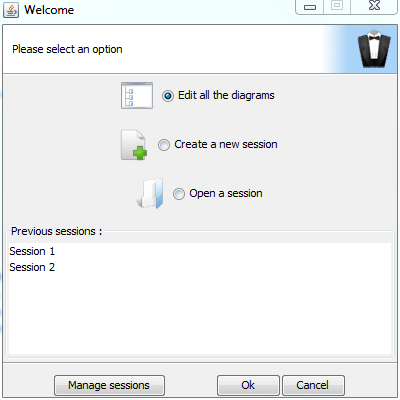
\includegraphics[width=0.4\textwidth]{../images/ouverture_session.png}
\caption{The session management interface is accessible from the welcome panel}
\end{figure}

\begin{figure}[h!]
\centering
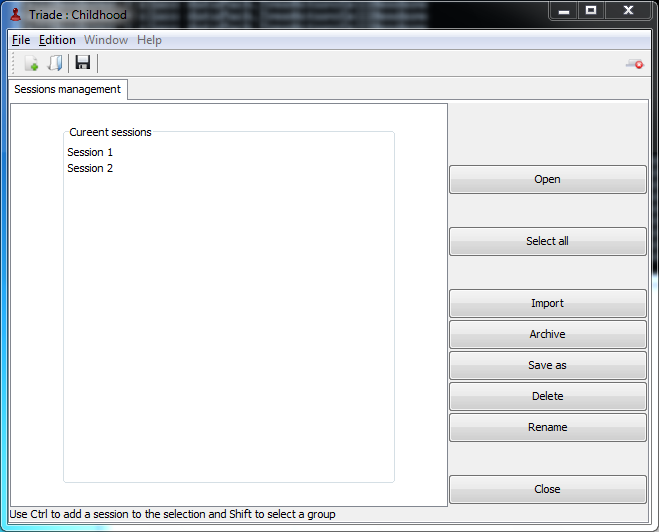
\includegraphics[width=0.8\textwidth]{../images/gestion_session.png}
\caption{The session management interface}
\end{figure}

\subsection{Default edge label}
It is possible to change the default edge label content. The sub-menu "Brick edge labels" allow the following possibilities : 
%Il est possible de changer le contenu par défaut des étiquettes des arêtes dans les briques. Le sous-menu "Etiquettes des arêtes des briques" dans le menu Edition. Les   différents contenus sont :\\
\begin{itemize}
\item \textbf{Structural relations} : Display the 4 first characters of structural relations for each action times.\\
%\item \textbf{Relations structurelles} : Affiche les 4 premiers caractères des relations structurelles de chaque temps d'action.\\
\item \textbf{Real relations} : The same with real relations.\\
%\item \textbf{Relations réelles} : De même avec les relations réelles.\\
\item \textbf{Relation at action time : *} : Display the structural and the real relations for the selected action time.\\
%\item \textbf{Relation au temps d'action : *} : Affiche la relation structurelle et la relations réelle pour le temps d'action sélectionné.\\ 
\end{itemize}

This setting affect only the edge labels in the bricks. In the exports, edge labels are controlled by the global export settings (see also section \ref{globalExport}).\\
%Cette option ne concerne que les relations dans les briques. Dans les exports, ces étiquettes sont contrôlées par les options globale de l'export (voir paragraphe \ref{globalExport}).\\

\begin{figure}[h!]
\centering
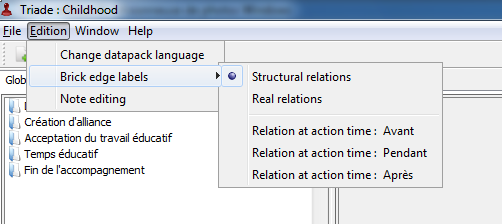
\includegraphics[width=0.5\textwidth]{../images/menu_edition.png}
\caption{The default edge label sub-menu}
\label{menu_edition}
\end{figure}

\subsection{Global export settings}
\label{globalExport}
The frame under the actor tree in the left of export window allow to control several settings which affect the whole export.\\
%Le cadre présent sous l'arbre des acteurs sur la gauche de la fenêtre permet de contrôler plusieurs éléments portant sur l'ensemble de l'export.\\

The first field is for editing the title of the export. If this field is let empty, the title will be hidden.\\
%Le premier champ permet de modifier le titre de l'export. Laisser ce champ vide masque le cadre de titre.\\

The next combo control the default edge label. The possibilities of the sub-menu "Brick edge labels" are available, but it is also possible to hide all unmodified labels with the "No label" option.\\
%Le champ suivant permet de modifier les étiquettes par défaut des arêtes. Il est possible de masquer l'ensemble des arêtes avec l'option "Aucune étiquette". Cela permet de n'afficher que les étiquettes des arêtes modifiées manuellement.\\

The next two fields control the default size of edge and vertex labels.\\
%Les deux champs suivants permettent de modifier la taille par défaut des étiquettes des sommets et des arêtes.\\

\begin{figure}[h!]
\centering
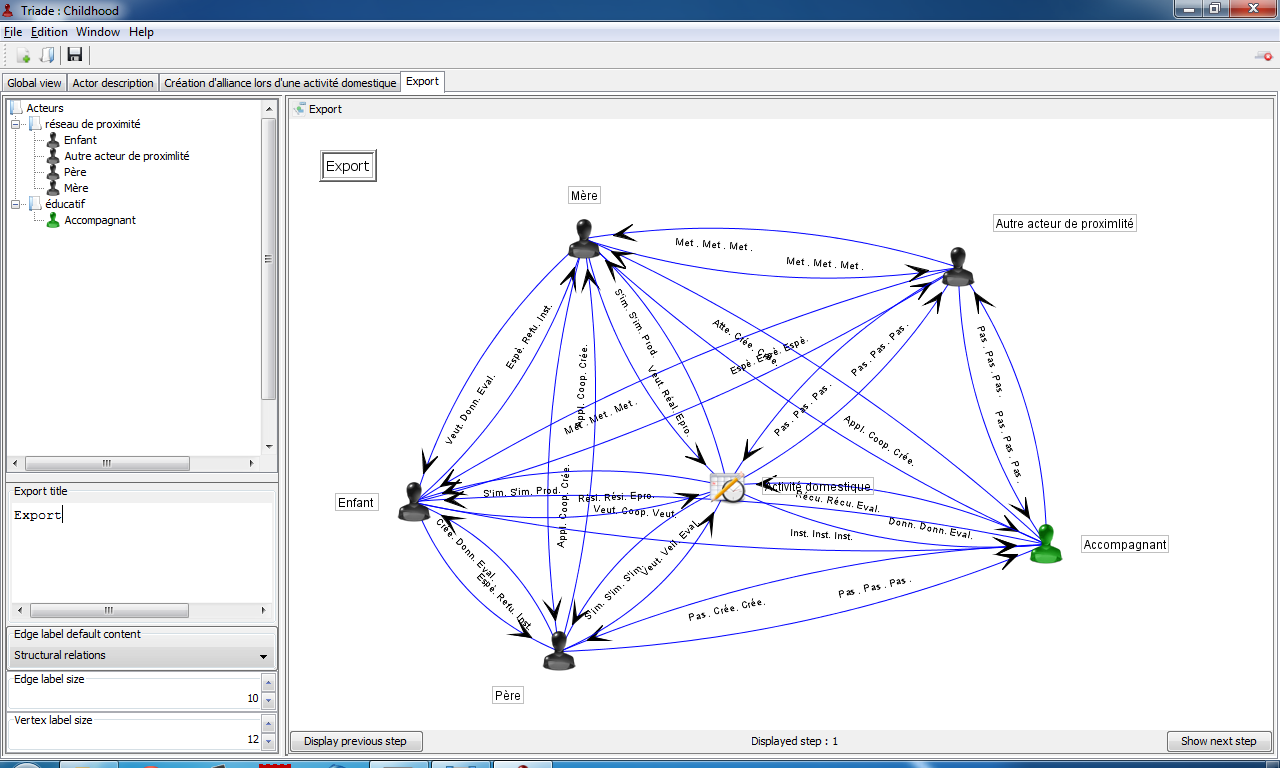
\includegraphics[width=0.5\textwidth]{../images/export_global.png}
\caption{The global settings frame is on the bottom left corner.}
\end{figure}


\subsection{Note editing in bricks}
Each brick is associated with a note. It is useful to keep information and to add some explanation for the situation described in the brick. By default, note are not editable. The option "Note editing" have to be selected to enable note editing. This option is in the edition menu (see picture \ref{menu_edition}). A note is associated to a session, it will be only accessible from the session in which it has been created.\\
%Chaque brique est maintenant associée à une note. Cela permet d'ajouter des informations pour décrire une situation. Par défaut, les notes ne sont pas éditables. Il faut activer l'option "Edition des notes" dans le menu édition avant de pouvoir les modifier (voir image \ref{menu_edition}).\\

Notes are displayed in the upper-right corner of the brick window. The note could be hidden or displayed by clicking on the arrow.\\
%Les notes sont accessibles à l'aide du cadre présent en haut à droite de la zone d'affichage d'une brique. Attention, les notes sont liés à une brique et à une session. En particulier, elles ne sont pas partagées entre les sessions.\\

\begin{figure}[h!]
\centering
\begin{subfigure}{0.4\textwidth}

\centering
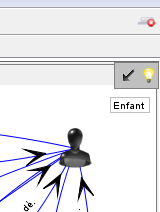
\includegraphics[width=0.4\textwidth]{../images/note_fermee.png}
\caption{A note in hidden mode}
\end{subfigure}

\begin{subfigure}{0.4\textwidth}

\centering
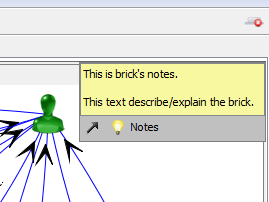
\includegraphics[width=0.8\textwidth]{../images/note_ouverte_pas_edition.png}
\caption{An openend note with editing mode disabled}
\end{subfigure}

\begin{subfigure}{\textwidth}

\centering
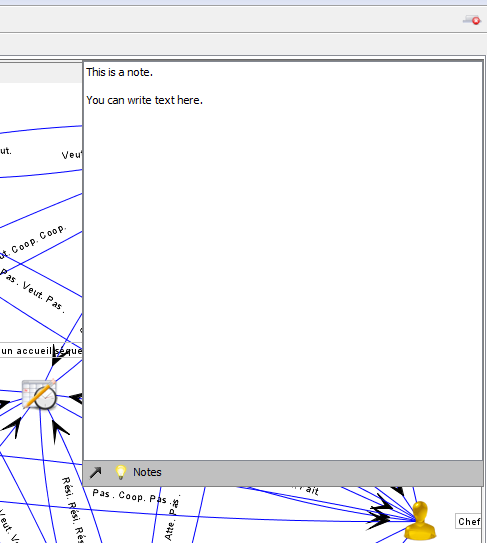
\includegraphics[width=0.4\textwidth]{../images/note_ouverte_edition.png}
\caption{An opened note with editing mode enabled}
\end{subfigure}


\end{figure}



\subsection{Datapack translation management}
It is possible to export and to import translation of the datapack. Use the corresponding buttons in the bottom of string translator interface \\
%Il possible d'importer et d'exporter une traduction depuis le module de traduction.\\

Warning, the current translation is lost when a new one is imported. Verify if you need to export before import the new one.\\
%Attention, lors d'une importation, la traduction est perdue. Veillez à exporter cette dernière avant si vous voulez la conserver.\\

It is also possible to change the translation from \tria with the option "Change datapack language" in the Edition menu (see picture \ref{menu_edition}). As in String translator module, the current translation will be lost.\\
%Il est aussi possible de changer la traduction depuis le datapack avec l'option "Changer la langue du datapack" dans le menu Edition (voir image \ref{menu_edition}). De même, la traduction actuelle sera écrasée lors de cette opération.\\

\begin{figure}[h!]
\centering

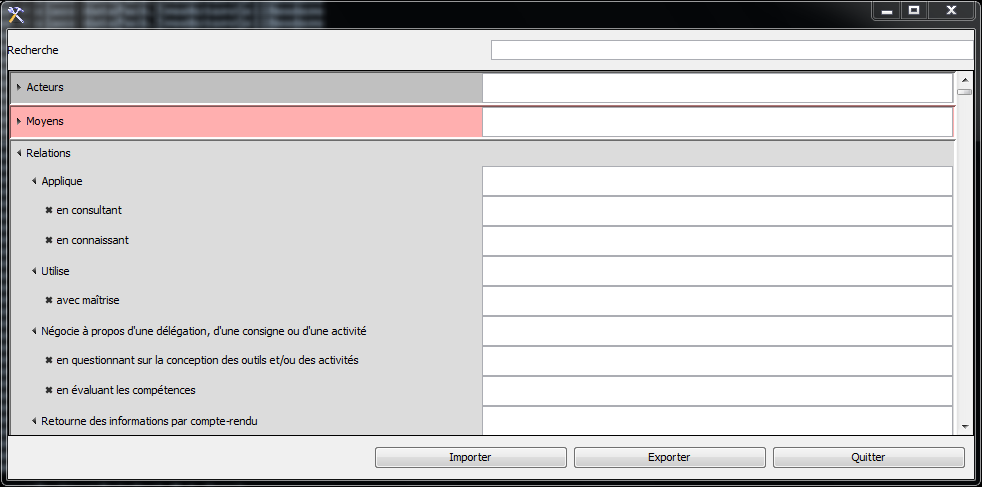
\includegraphics[width=0.8\textwidth]{../images/translator.png}
\caption{The string translator interface.}
\end{figure}



\section{Version 1.0.2}
\subsection{Translation statistics}

The button "Translation statistics" in the bottom left of the window display the count of translated words and sentences.\

\subsection{Export deletion}
It is possible to delete an export with a right click on it in the global view. The export will stay in the list until the next launch of the software.\\

\section{Version 1.0.3}



\subsection{Selection of software interface language}
The language of software interface can be changed with the "Language" menu in the main window. The software needs to be restarted after a change of language.
%La langue de l'interface peut être choisie à l'aide du menu "Langue" dans l'interface principale. Le logiciel doit être redémarré après un changement de langue.\\

It is possible to add a new language by adding the corresponding file in the sub-folder "language" in the installation \tria folder. To do so, make a copy of any other language file, rename it with the correct code and translates every sentences in the file. The new language will be automatically added to the list of available language in the "Language" menu.\\
%Il est possible d'ajouter une nouvelle langue en ajoutant le fichier correspondant dans le sous dossier "language" du répertoire d'installation du logiciel. Pour réaliser cette traduction, il suffit de réaliser une copie d'un des fichier puis de traduire l'ensemble des phrases qu'il contient. La nouvelle langue sera proposée dans le menu "Langue" lors du démarrage suivant du logiciel.\\

If some sentences are not translated in the software, that could comes from missing sentences in the translation file. In this case, french translation is used instead. That could be corrected by adding the missing sentences in the corresponding file in the language folder.\\
%Si des phrases sont manquantes dans un fichier de traduction, celles de la version françaises seront automatiquement utilisées à la place. De ce fait, si certaines phrases sont en français, cela signifie sûrement que leur traduction est manquante. 


\subsection{Automatic datapack download and update}
During the first launch of student version of \tria, the user have to enter the address to download the datapack. Indeed, the student version installer does not contains a datapack in order to allow a easier distribution of sessions and local datapack translation. It is possible that the software needs to be restarted after the downloading of the datapack file.\\

%Lors du premier lancement de la version étudiante, l'utilisateur est invité à saisir une adresse à laquelle le datapack peut être téléchargé. En effet, le logiciel en version étudiante est initialement fourni sans datapack afin de permettre un déploiement plus aisé de nouvelles sessions ou d'une traduction locale du contenu du datapack. Il est possible qu'il soit nécessaire de relancer le logiciel une fois le fichier téléchargé.\\

\subsubsection{AutoUpdater software}
The software "AutoUpdater" do an automatic update of the datapack from a file downloaded from internet.\\
%Le programme "AutoUpdater" permet de mettre à jour automatiquement le datapack à partir d'un fichier téléchargé sur internet.\\

When "AutoUpdater" is launched, the user have to input the address where the datapack could be downloaded. When the old datapack and the new one contains a translation or some sessions sharing the same name, the user is asked about which version he wants to keep.\\
%Lors du lancement de l'autoUpdater, l'utilisateur est invité à saisir l'adresse de téléchargement du datapack. Dans le cas où le datapack courant et le nouveau contiennent une traduction ou des sessions portant le même nom, le programme demande à l'utilisateur quelle version il souhaite conserver.\\

A backup of the old datapack is automatically done, the backup file is placed in the sub-folder "datapack\_backup".\\
%Une sauvegarde de l'ancien datapack est automatiquement réalisée et placée dans le dossier "datapack\_backup".


\subsection{License management}
Datapack used with student version have a limited trial time. When buying a use license, an unlocking code is given. This code could be entered in the software with the option "Register a license" in the "Help menu". A dialog pop-up, to request the mail address associated with the license and the registration code.\\

%Les datapacks fournis avec la version étudiante du logiciel ont un durée d'utilisation limitée dans le temps. Lors de l'achat d'une licence, un code de déblocage du datapack est fourni. Ce code peut être saisi à l'aide de l'option "Enregistrer une licence". Une fenêtre s'ouvre alors invitant l'utilisateur à saisir l'adresse mail associée à la licence puis le code de validation.\\

When the software is launched with an expired datapack, a dialog pop-up to request from the user his license information. The software could need to be restarted after registering a license. 
%Lors de l’utilisation d'un datapack dont la durée d'essai s'est achevé, une boite de dialogue invite l'utilisateur à saisir ces mêmes informations pour permettre l'utilisation du datapack. Il est possible qu'un redémarrage du logiciel soit nécessaire lors de la saisie d'une licence.\\




\subsection{Teachers version features}
\subsubsection{Licenses generation and limited time datapack}

The "Tools" menu, only available in the teacher version, allow user to generate use-licenses and limited time datapack for student version. 
%Le menu "Outils", uniquement présent dans la version enseignant du logiciel, permet de générer des licences d'utilisation ainsi que d'exporter des datapack à destination des versions étudiantes.

Those two tools request user to enter his personnal key. This key has been normally given to you during software distribution. If not, please contact developpers team.\\
%Lors de l'utilisation de ces deux outils, il vous est demandé de saisir votre clé personnelle. Cette dernière vous a normalement été fournie lors de la livraison du logiciel.\\

\paragraph{Licenses generation}

The first step of licenses generation is to enter the list of mail address for which a license needs to be generated. This list could be extract from the clipboard, the mail address should be separated by ',' or ';' or a tabulation or a line jump. This function allow to import the list from a spreadsheet software.\\
%La génération de licences se déroule en deux étapes. Tout d'abord, l'utilisateur doit saisir la liste des adresses mails pour lesquelles une licence doit être générée. Il est possible d'extraire cette liste depuis le presse-papier. Dans ce cas, les séparateurs utilisés sont au choix : la virgule, le point-virgule, la tabulation et le retour chariot. Cela permet en particulier d'importer facilement cette liste depuis un tableur.\\

It is also possible to add an address with the dedicated field and button in the top of the window. Entries can be modified or deleted with the button on the top right of the window.\\
%Il est aussi possible d'ajouter une adresse à l'aide du champ mail et du bouton juste à sa droite situé en haut de la fenêtre. Les différentes entrées pouvant être modifiées et supprimées à l'aide des boutons dédiés en haut à droite de la fenêtre.\\

License type could be selected with the radio-button list on the bottom of the window. It is not possible to specify different licence for a same list. The option "Already billed licenses" allow to regenerate an unlock key for an user who have lost his key.\\
%Le type de licence peut être choisi à l'aide de la liste à puce en bas de la fenêtre. Il n'est pas possible de spécifier plusieurs licences différentes pour une même liste. L'option "Licence déjà facturée" permet de générer à nouveau un code de licence au cas ou ce dernier aurait été perdu par l'utilisateur.\\

The next step is to generate licences. Warning, an internet connection is requested during this step. The process is launched with the button "Generate licences" in the bottom right of the window. The mail list won't be editable further.\\
%L'étape suivante consiste à générer les licences. Attention, un connexion internet sera nécessaire lors de cette étape. Le processus est lancé lors du clic sur le bouton "Générer les licences". La liste de mail ne sera plus modifiable par la suite.\\

The user have to select the file which a summary of all generated licenses have to be saved. Then , it is possible to copy a mail address, an unlock key, a couple mail/key or the while list with the buttons on the right of the window.\\
%L'utilisateur est invité à choisir le lieu d'enregistrement du fichier de licence dans lequel il veut stocker le récapitulatif des licences générés. Il est ensuite possible de copier au choix une adresse mail, un code de déblocage, un couple mail/code de déblocage ou la liste entière à l'aide des boutons situés sur la droite de la fenêtre.\\

Once the window has been closed, it is not possible to access to the generated key list in the software, but only by the summary file saved during the process.\\
%Une fois la fenêtre de génération des licences fermées, il n'est plus possible d'accéder à la liste générées au sein du logiciel, mais uniquement grâce au fichier récapitulatif créé lors de la génération.\\


A billing request will be automatically send to the software dealer during licenses generations.\\
%Une demande de facturation est automatiquement envoyé à l'équipe de développement lors de la génération des licences.


\paragraph{Generation of limited time datapack for student version}%Génération d'un datapack pour les version étudiantes}

The other option of tools menu allow to generate trial datapack. In this purpose, the user has to enter the trial period duration. The maximum is 365 days, and the minimum is 0. The trial period start on the datapack generation day. If the value 0 is used, the datapack will be always locked. It is usefull for user who had bought a license and who needs to reinstall the software. They can download a datapack of this kind and then unlock it whit their license key.\\
%L'autre option du menu outils permet de générer des datapack pour les versions étudiantes du logiciel. Lors de cette opération, l'utilisateur est tout d'abord invité à saisir la durée de validité du datapack. La durée maximale est de 365 jours. La durée minimale est 0 jours, cela correspond à un datapack bloqué immédiatement. Ce type de datapack est destiné à être mis à disposition des utilisateurs ayant acheté une licence d'utilisation afin qu'(il puisse le télécharger lors d'une réinstallation ultérieure du logiciel.\\

After setting the trial duration, the user have to select where to save the trial datapack. Then, the datapack will be automatically exported.\\
%La fenêtre suivante invite l'utilisateur à choisir l'endroit ou le datapack devra être enregistré.\\

%Une fois l'emplacement choisi, le datapack est automatiquement exporté.\\


\end{document}
